%!TEX root = thesis.tex


%
%==========================================================================================
%
\chapter{Security Domain}
\label{chap:civabis}

% 
\includepdf[pages=2-last, fitpaper=true, addtotoc={
% 2, section, 1, {A Probabilitic Risk Analysis for Multimodal Entry Control}, sec:eswa, %
% 2, subsection, 2, {Introduction}, sec:eswa:intro, %
% 3, subsection, 2, {Related Work}, sec:eswa:related, %
% 3, subsection, 2, {Hierarchical Multimodal Framework}, sec:eswa:framework, %
% 	3, subsubsection, 3, {Functional Description}, sec:eswa:framework:desc, %
% 	4, subsubsection, 3, {Architecture}, sec:eswa:framework:architecture, %
% 	4, subsubsection, 3, {Observing the person's behavior}, sec:eswa:framework:observing, %
% 	4, subsubsection, 3, {Experimental Environment}, sec:eswa:framework:environment, %
% 	5, subsubsection, 3, {Ontology}, sec:eswa:framework:ontology, %
% 5, subsection, 2, {Modules and Algorithms}, sec:eswa:modules, %
% 	5, subsubsection, 3, {Expert Rules}, sec:eswa:modules:rules, %
% 	6, subsubsection, 3, {Micro Learning}, sec:eswa:modules:micro, %
% 	6, subsubsection, 3, {Macro Learning and Meta-Learning}, sec:eswa:modules:macro, %
% 	7, subsubsection, 3, {Visual Learning}, sec:eswa:modules:visual, %
% 	7, subsubsection, 3, {Integration}, sec:eswa:modules:integration, %
% 8, subsection, 2, {Experimental Results}, sec:eswa:experiments, %
% 	8, subsubsection, 3, {Learning Phase}, sec:eswa:experiments:learning, %
% 	8, subsubsection, 3, {Evaluation Phase}, sec:eswa:experiments:evaluation, %
% 9, subsection, 2, {Discussion and Conclusion}, sec:eswa:conclusion, %
% 9, subsection, 2, {References}, sec:eswa:references %
% }]{article/ESWA5529.pdf}

Entry control is an important security measure that prevents undesired persons from entering secure areas. The unified detection framework utilized in this chapter allows an advanced risk analysis to distinguish between acceptable and unacceptable entries, based on several entry sensors, such as fingerprint readers, and intelligent methods that learn behavior from previous entries. First, it analyzes person behavior from different viewpoints and then performs a joint risk analysis. The obtained results represent an improvement in detecting security attacks.

%%%%%%%%%%%%%%%%%%%%%%%%%%%%%%%%%%%%%%%%%%%%%%%%%%%%%%%%%%%%%%%%%%%%%%%
%
% I N T R O D U C T I O N
%
%%%%%%%%%%%%%%%%%%%%%%%%%%%%%%%%%%%%%%%%%%%%%%%%%%%%%%%%%%%%%%%%%%%%%%%

\section{Introduction and Background}

Building and system safety and integrity have become more important due to the increased threat of terrorist attacks, system intrusions, and frauds. An important security requirement is to ensure effective entry controls that prevent unauthorized persons from accessing specific areas. 

The general approach is to combine a two-stage security check: the identification stage, where the person introduces his/her identity; and the verification stage, based on a password and/or one or more signals derived from physical traits, such as fingerprint, voice, iris or written signature. Although widely used, entry control has certain weaknesses in the real world. Classic security methods fail to recognize unauthorized access if, for example, an identification card is stolen, a fingerprint is faked, or an employee is forced to open the door for unauthorized persons. 
%Furthermore, a human supervisor or guard is not able to effectively control a variety of access points for several hours and can be fooled even by simple tricks.
However, intelligent access-control systems offer the promise of improved performance at a reasonable cost.

A common practice in most reported studies is to improve the two-stage security by (i) using advanced biometric methods \citep{Wahyudi2007, Wong2009, Sun2008}; (ii) analyzing behavior \citep{Zhang2007, Lin2008, Quah2008, Alexandre1997, wilson2006, Stephen2005, Depren2005}; or (iii) combining multiple sensors into a single, reliable estimation \citep{lamborn2006, Bontempi2005, Fierrez-Aguilar2005}. In all the above-referenced studies, the methods successfully reduced the risk of intrusion, although each approach was focused on one specific viewpoint. \citet{Wahyudi2007}, for example, presented a verification based on speech analysis. They constructed voice-based models for authorized persons and performed the identification with an adaptive network-based fuzzy-inference system. In a similar way, \citet{Wong2009} and \citet{Sun2008} focused on face recognition. Various facial features were extracted from video, saved in a database and compared with a new entry. The authors report an accuracy of over 90\%.

Recent research efforts have focused on meta-learning \citep{Brazdil2009, Vilalta02, Wang1997}. The basic objective is to consider various aspects and hypotheses about an event and the environment to construct a situational awareness;  then, on this basis, risk is reliably estimated. \citet{lamborn2006} introduced an intelligent system that consists of several heterogeneous sensors divided into clusters according to their GPS location using self-organizing maps. Sensor outputs are classified into each cluster and a voting algorithm is used to compute the final classification. Several data-mining methods were tested for cluster classification; for example, k-NNs, neural networks, and SVMs. A similar system was presented by \citet{Bontempi2005}. In addition, \citet{Fierrez-Aguilar2005} exploited person-specific multimodal biometric parameters. They proposed an adapted local learning scheme (person-de\-pen\-dent) and global learning scheme (person-in\-de\-pendent), with both results fused with weighted voting. The authors reported that the adapted learning outperformed the results from single learning.


The described approaches use state-of-the-art methods that successfully reduce intrusion risk. They use additional biometric sensors and behavior analyses as upgrades to classic access control. Our approach is a further step in combining an arbitrary number of methods in three stages. In the first stage, an arbitrary number of intelligent modules is utilized, with analyzing person behavior from different viewpoints and performing its own risk analysis. Similar to \citet{lamborn2006}, our system constructs a situational awareness from different sensors, but, in contrast to their method, the intelligent module outputs in the second stage are assembled using meta-learning, on top of which the final reasoning is performed with a Bayesian network. In addition, the intelligent modules utilize both person-specific parameters and global knowledge similar to \citet{Fierrez-Aguilar2005}, but the last integration is fused proficiently. Finally, the system is also able to explain the evaluations to a human operator and helps him/her to understand the situation. The basic assumptions of our approach are that (i) person behavior rarely changes significantly over time, and (ii) combined methods are much harder to bypass than a single sensor or method.

%The rest of this chapter is structured as follows. Related work is described in detail in Section~\ref{sec:relatedWork}. The general structure of the proposed framework is presented in Section~\ref{sec:system}, while Section~\ref{sec:modules} describes the individual modules and the final integration in detail. Section~\ref{sec:results} presents the experimental evaluation and results with an on-line adversary test. Finally, Section~\ref{sec:conclusion} summarizes the work done and concludes the chapter with a discussion.


%%%%%%%%%%%%%%%%%%%%%%%%%%%%%%%%%%%%%%%%%%%%%%%%%%%%%%%%%%%%%%%%%%%%%%%
%
% R E L A T E D   W O R K
%
%%%%%%%%%%%%%%%%%%%%%%%%%%%%%%%%%%%%%%%%%%%%%%%%%%%%%%%%%%%%%%%%%%%%%%%


%%%%%%%%%%%%%%%%%%%%%%%%%%%%%%%%%%%%%%%%%%%%%%%%%%%%%%%%%%%%%%%%%%%%%%%
%
% S Y S T E M
%
%%%%%%%%%%%%%%%%%%%%%%%%%%%%%%%%%%%%%%%%%%%%%%%%%%%%%%%%%%%%%%%%%%%%%%%

\section{Hierarchal Multimodal Framework}
\label{sec:system}

%\subsection{Functional Description}
%\label{sec:system:description}

The aim of our system is to ensure increased security in critical areas, such as military headquarters or political institutions, by detecting irregular accesses or unusual access point behavior, and, on this basis, raising an alarm. In order to reduce intrusion risk, we have designed a modular system that relies heavily on intelligent methods.

\subsection{Functional Description}
\label{sec:system:description}

The entry procedure is shown in Figure~\ref{fig:procedure} and is as follows: first, a person is identified. Next, if his/her identity exists, the person is verified, which leads to the door lock being released. The verification process is performed in two stages: a classic biometric verification, and an intelligent verification. Intelligent modules evaluate the entry and suggest the proper action.

\begin{figure}[!ht]
\centering
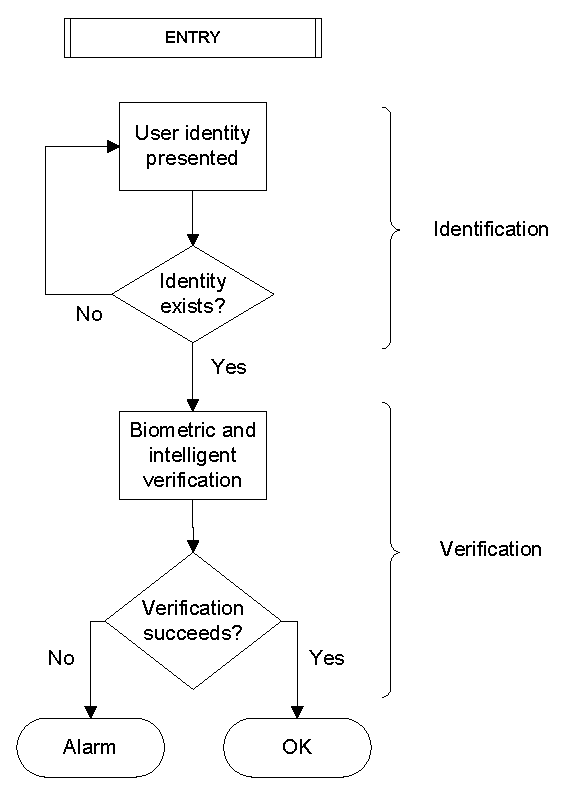
\includegraphics[width=0.6\linewidth]{chap_security/entry}
%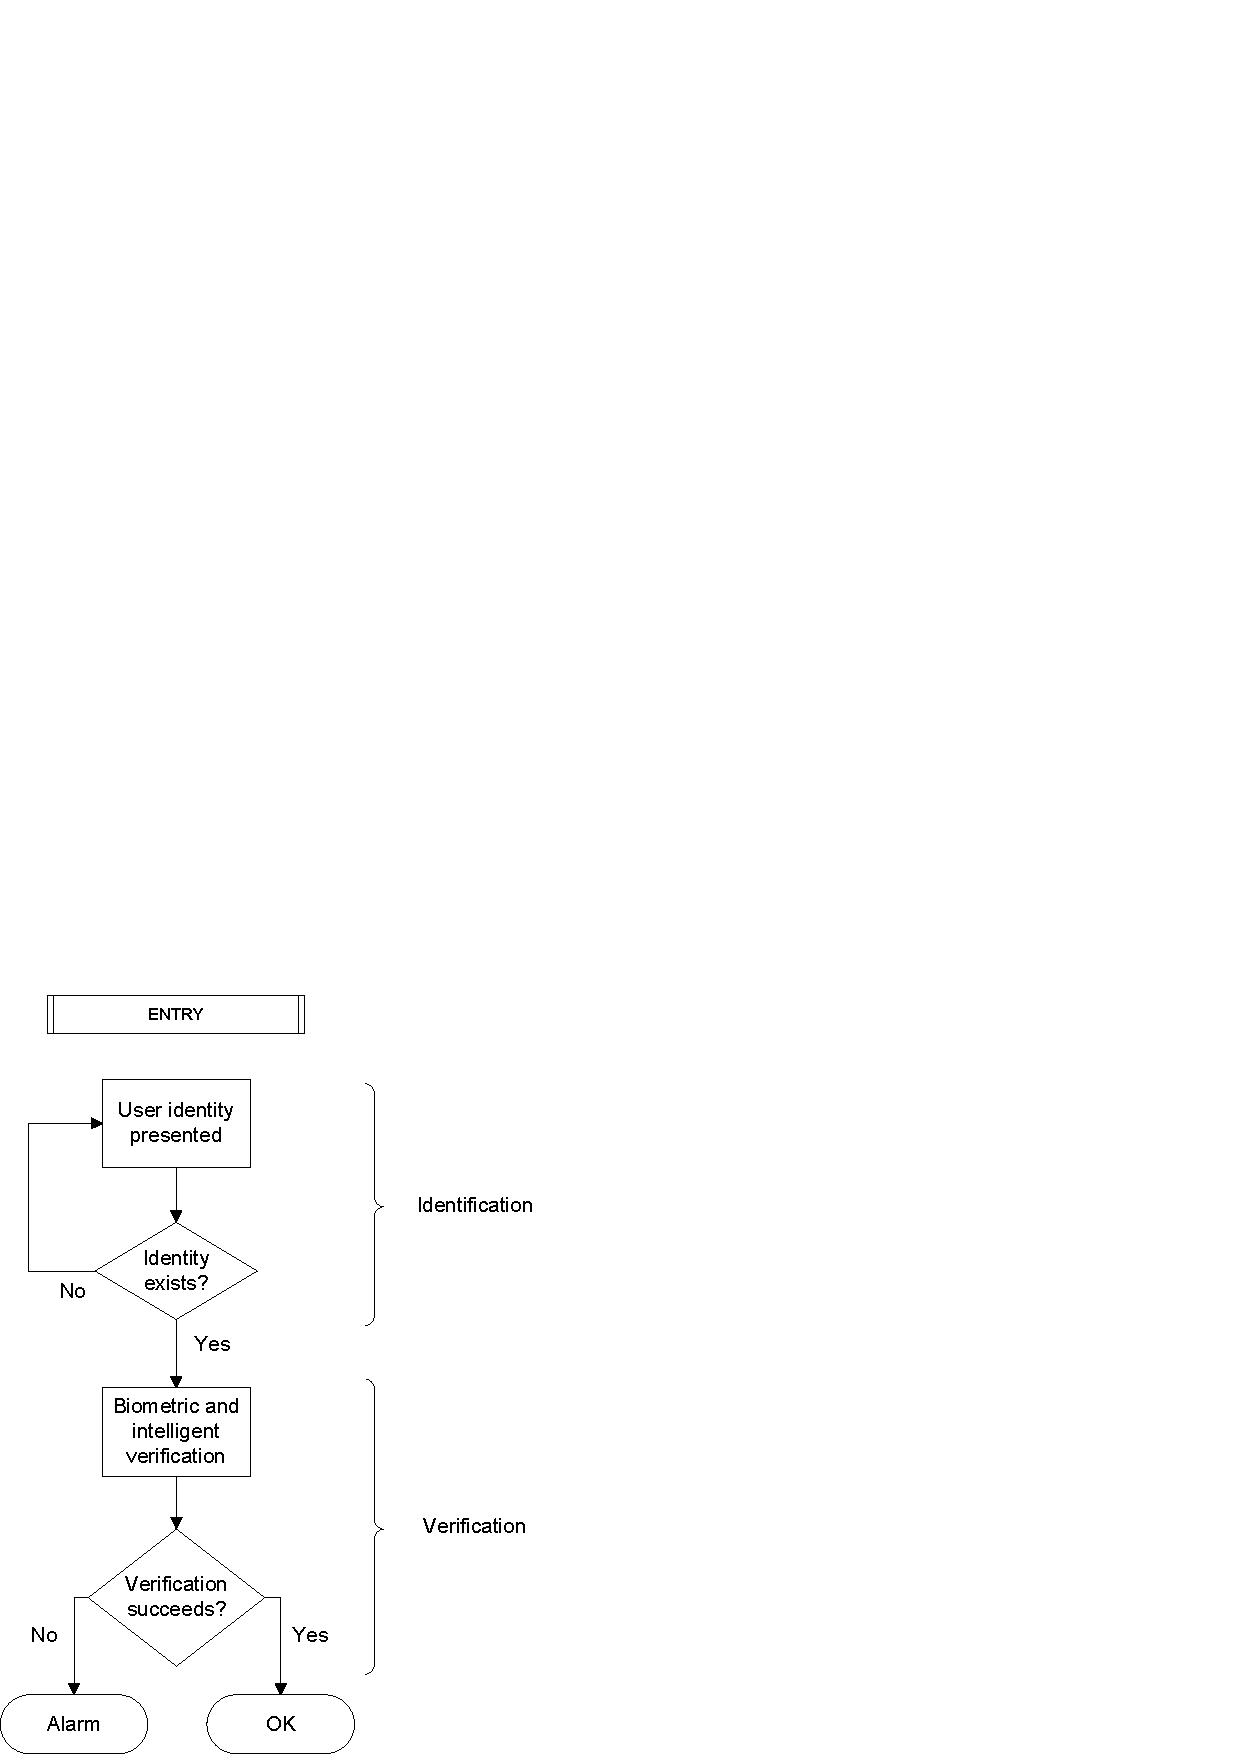
\includegraphics[bb=100 230 380 600, width=8cm]{chap_security/entry.pdf}
\caption{Entry identification and verification procedure at a high-secured access point.}
\label{fig:procedure}
\end{figure}

The proposed intelligent access-control system's development was based on the following five requirements: first, the system must monitor entries and process evaluations in real time. Second, several access points may need to be monitored at the same time, taking into account knowledge of the person's movement between them. Third, an arbitrary number of sensors and intelligent modules will be used, depending on the equipment at specific access points and data availability. Fourth, the system is expected to evaluate an entry and suggest the proper action. Finally, the system should explain its evaluation in a user-friendly, interactive control panel. In short, the aim is to create a system that will improve entry control security and help the operator to control numerous access points effectively. 


\subsection{Architecture}
\label{sec:system:architecture}

\index{unified framework}
The main architectural tasks are collecting the data from the peripheral devices and sensors, processing and analyzing this data, integrating the analyses into a human-readable form, and displaying them to a person with a suggestion for an appropriate action (Figure~\ref{fig:architecture}). 


\begin{figure}[!ht]
\centering
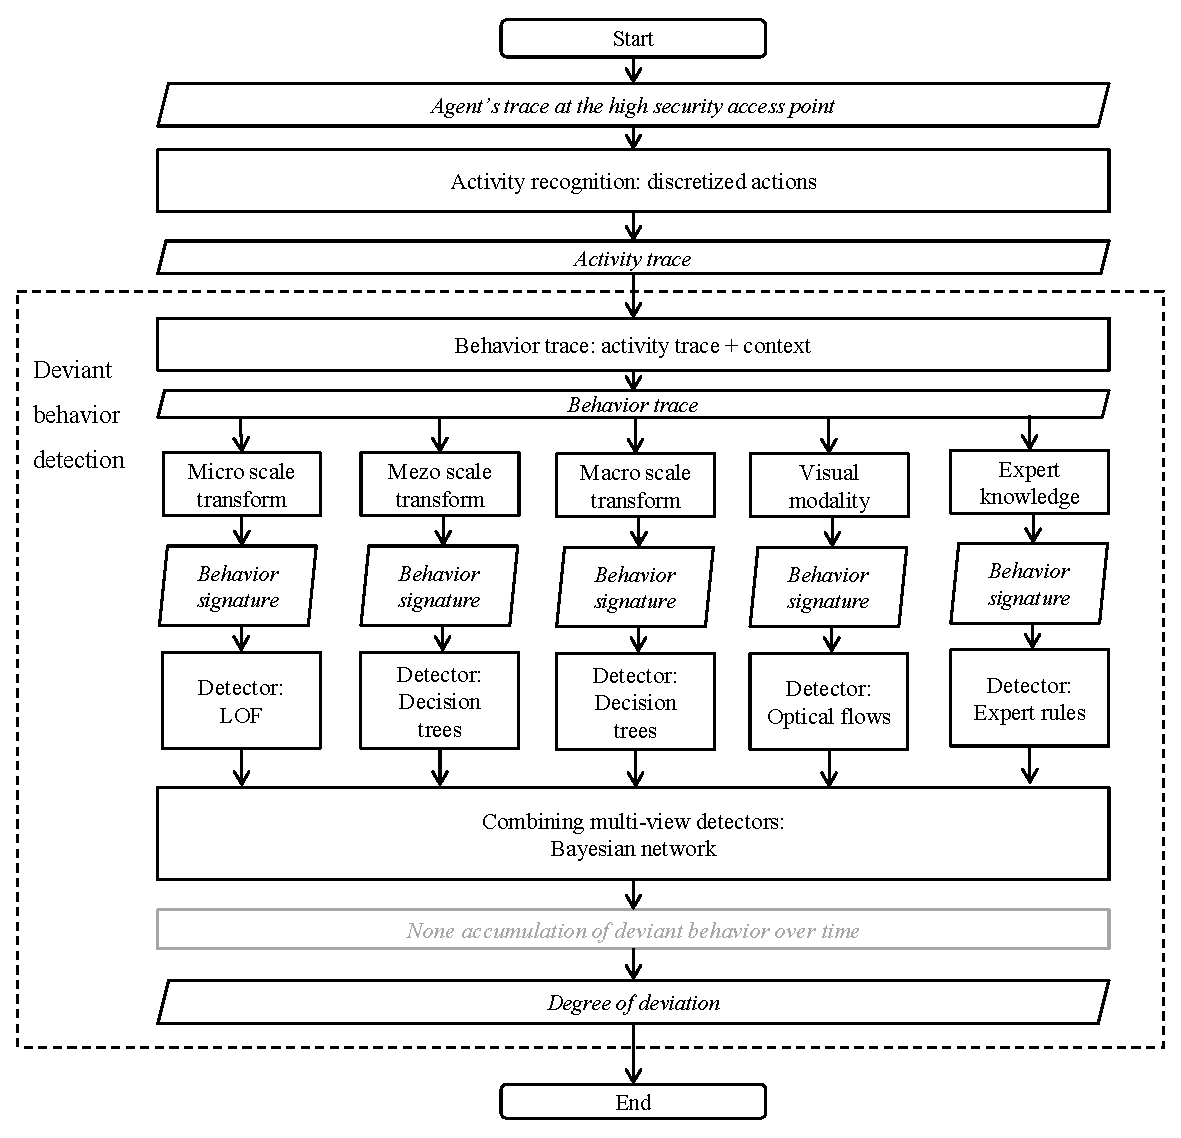
\includegraphics[width=1\linewidth]{chap_security/stack-SEC}
%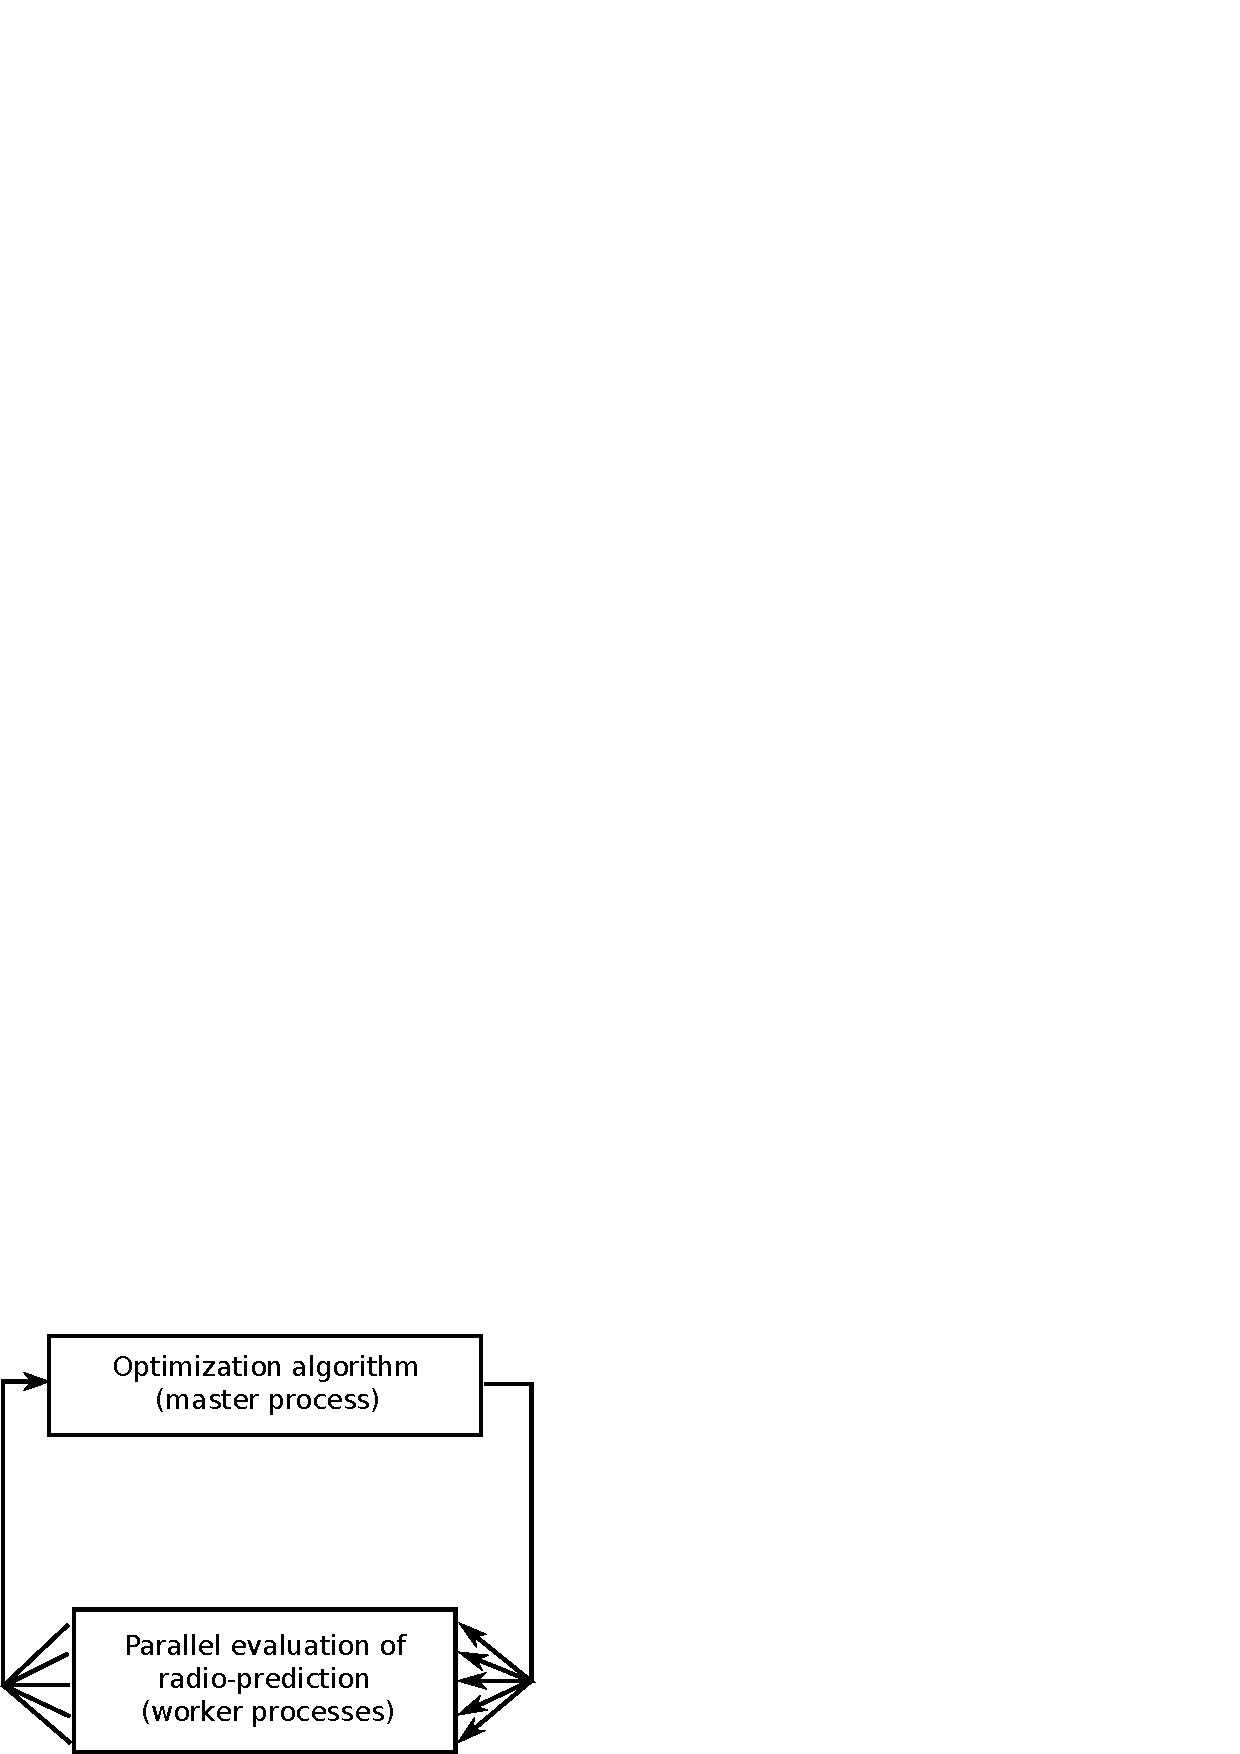
\includegraphics[bb=80 410 470 780, width=8cm]{chap_security/architecture.pdf}
\caption{Flowchart of the instantiated unified framework using multiple time scales and modalities to evaluate behavior.}
\label{fig:architecture}
\end{figure}

% \begin{figure}[]
% \centering
% 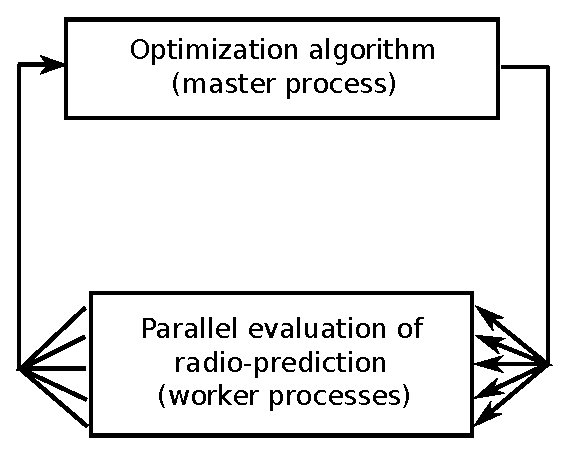
\includegraphics[width=0.8\linewidth]{chap_security/architecture}
% %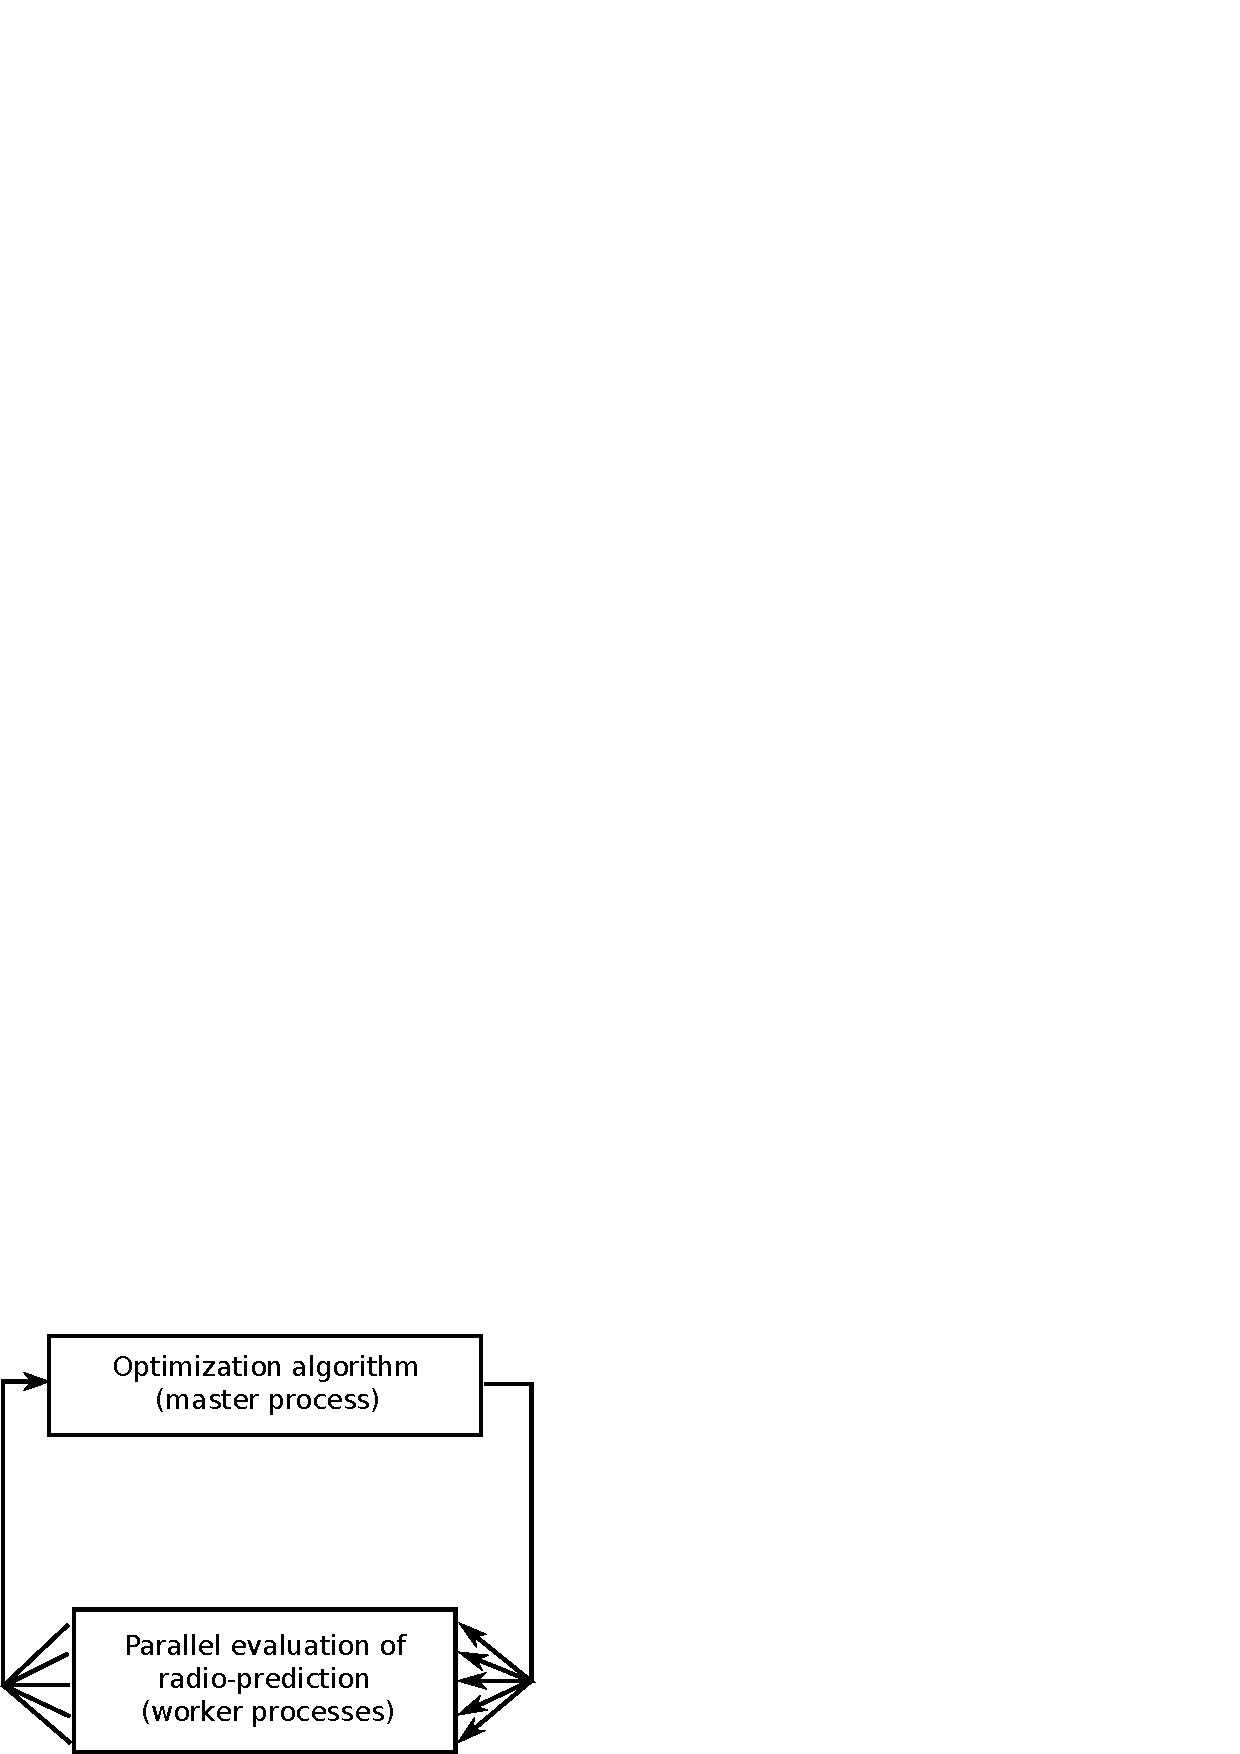
\includegraphics[bb=80 410 470 780, width=8cm]{chap_security/architecture.pdf}
% \caption{General architecture of the system. Our contribution is in gray.}
% \label{fig:architecture}
% \end{figure}


The system's architecture is designed in eight layers. In the first layer, various access point sensors are deployed, such as biometric sensors, visual sensors, or door opened/closed sensors. The sensors' output is captured in the next layer through a controller, providing an observation vector $\mathbf{x}_t$ at time step $t$, augmented with additional contextual information.

\index{activity recognition}
The activity recognition layer is simplified to recognizing $\mathbb{A}=\{entry, other\}$. If all the formal criteria are met, that is, the observation consists of all the required elements, then the activity is marked as \textit{entry} and evaluated as shown in Figure~\ref{fig:procedure}; otherwise, the entry is not completed and an alarm is raised immediately.

The next three levels are implemented in several parallel instances. Each instance constructs its own behavior patterns from a specific data type, such as visual data or temporal relations,  and applies an intelligent method to evaluate the behavior. The methods include decision trees, outlier detection, expert rules, computer vision and others. Finally, all previous parallel detector outputs are gathered and the system outputs the final evaluation using a Bayesian network.


\subsection{Observing the User's Behavior}
\label{sec:system:behavior}

Each human tends to perform activities in a specific way, be it on micro-or macro-scale. However, the person behavior in our system is actually monitored from three different points of view. In the first of these, denoted as the \textit{micro-level}, one typically deals with behavior that changes in seconds or tenths of a second. For example, one person always carries his identity card in a wallet and puts the whole wallet near the wireless identity-card reader, while another person carries her card in a handbag and requires some time to take it out, identify herself, and put the card back. The person's movement around the access point depends on his/her habits and mental/physical state. These facts determine the persons' micro-level patterns.

The second viewpoint, denoted as the \textit{macro-level}, describes the persons' daily routines. The activities are the access point arrival times, the movements between various access points in the access-control network, and even the connections between persons; for example, person $A$ often enters a short time after person $B$. The time scale used at the macro-level can vary from seconds to months.

The third viewpoint, denoted as the \textit{visual level}, captures the persons' access point visual movement using a camera. It is also focused on micro-level movements; that is, behavior that changes over a short time interval. However,  in addition to micro-level features, it obtains visual characteristic features of the person and his/her movement; for example, the person's height and the door-opening dynamics.

Several rules additionally control the regular entry procedure, the regular working time, and access permissions.


\subsection{Experimental Environment}
\label{sec:system:experimental}

To design and test our intelligent access control modules, we set up the experimental environment shown in Figure~\ref{fig:environment}, which consisted of a single access point protecting an office in a building. The access point was equipped with a camera (on the ceiling), a card reader and a fingerprint reader (on the wall near the door), an electronic lock, and an open/close sensor on the door. The input signals were collected with a multi-channel access controller connected to various peripheral devices. 
%Such controllers can be dynamically combined in order to ensure the centralized data management of sensors covering a complete access-control network. However, for our purpose, one controller was sufficient.

\begin{figure}[!ht]
\centering
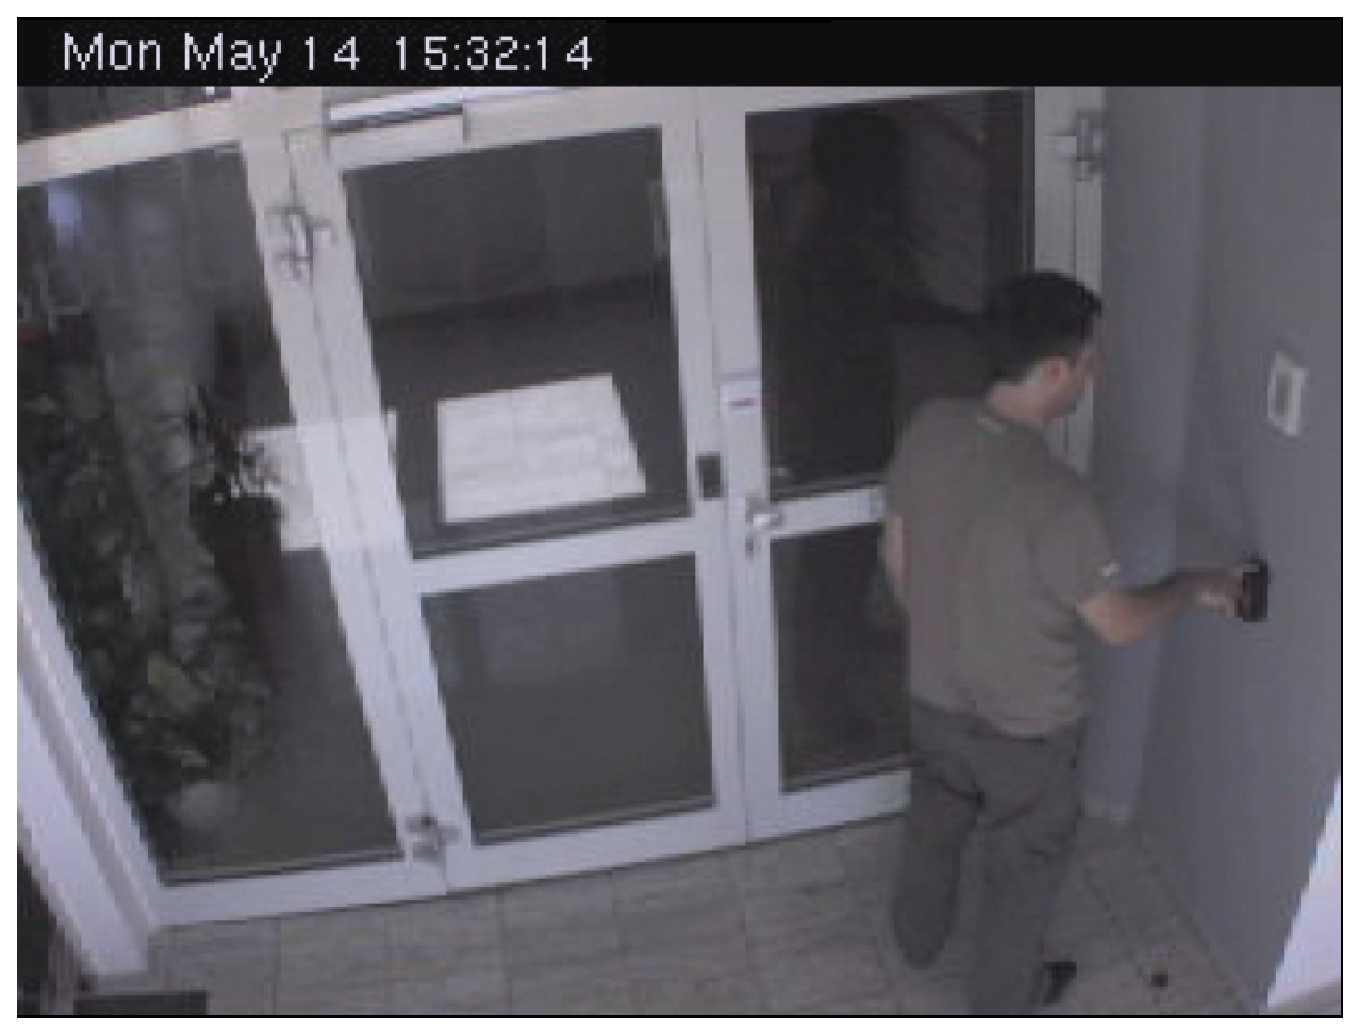
\includegraphics[width=0.8\linewidth]{chap_security/soba}
\caption{Prototype access-point configuration (camera view). The task is to detect suspicious entries of persons, for example, under the influence of drugs or with a gun that is outside the camera's field of view.}
\label{fig:environment}
\end{figure}

When a person passed the access point, four different times were registered:
\begin{itemize}
    \item	$t_c$ -- time of card-reader acceptance,
    \item	$t_f$ -- time of fingerprint-reader acceptance,
    \item	$t_{do}$ -- time of door opening,
    \item	$t_{dc}$ -- time of door closing.
\end{itemize}
The data was collected and written into the ontology for additional processing by six intelligent modules. The first module, denoted as the \textit{expert rules}, detected prohibited and basic undesired behavior. It used SWRL rules to query the system ontology (see Section~\ref{sec:modules:rules}). The second module, \textit{micro-learning}, learned person micro-level behavior patterns during the entry. The learning was performed with a local outlier-detection me\-thod (LOF) (described in more detail in Section~\ref{sec:modules:micro}). The three  \textit{macro-learning} modules learned the macro-level access patterns and were then combined at the meta-level (see Section~\ref{sec:modules:macro}). The last module, \textit{visual learning}, used optical flow histograms to detect visual-level behavior patterns (see Section~\ref{sec:modules:visual}).

Each module performed its own entry risk analysis and then returned an evaluation with an explanation. The meta-module used basic weighted voting based on single-module decisions, while the integration module accepted the module classifications as observations and performed the reasoning with a Bayesian network. 

\begin{figure}[]
\centering
%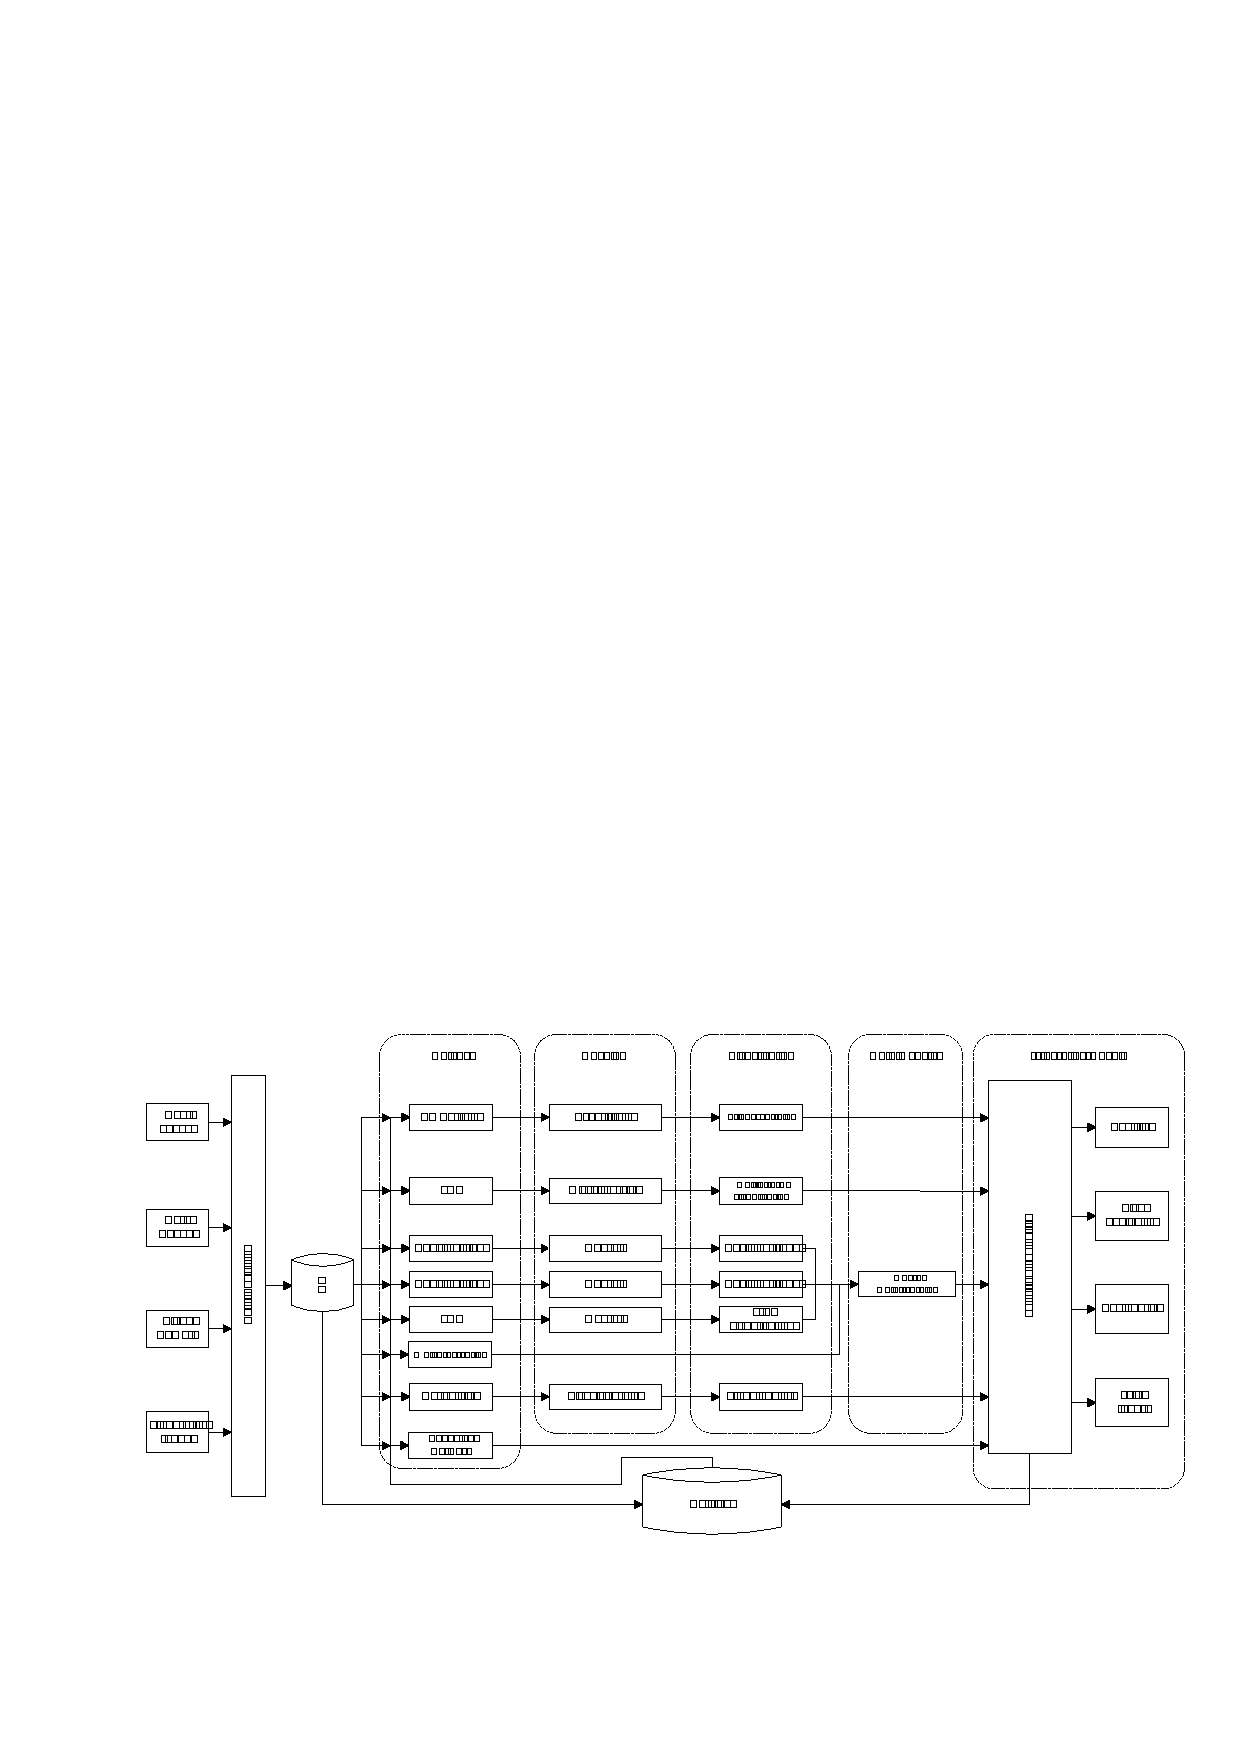
\includegraphics[bb=60 100 570 350, type=eps,ext=.eps,read=.eps,width=18cm]{chap_security/shema}
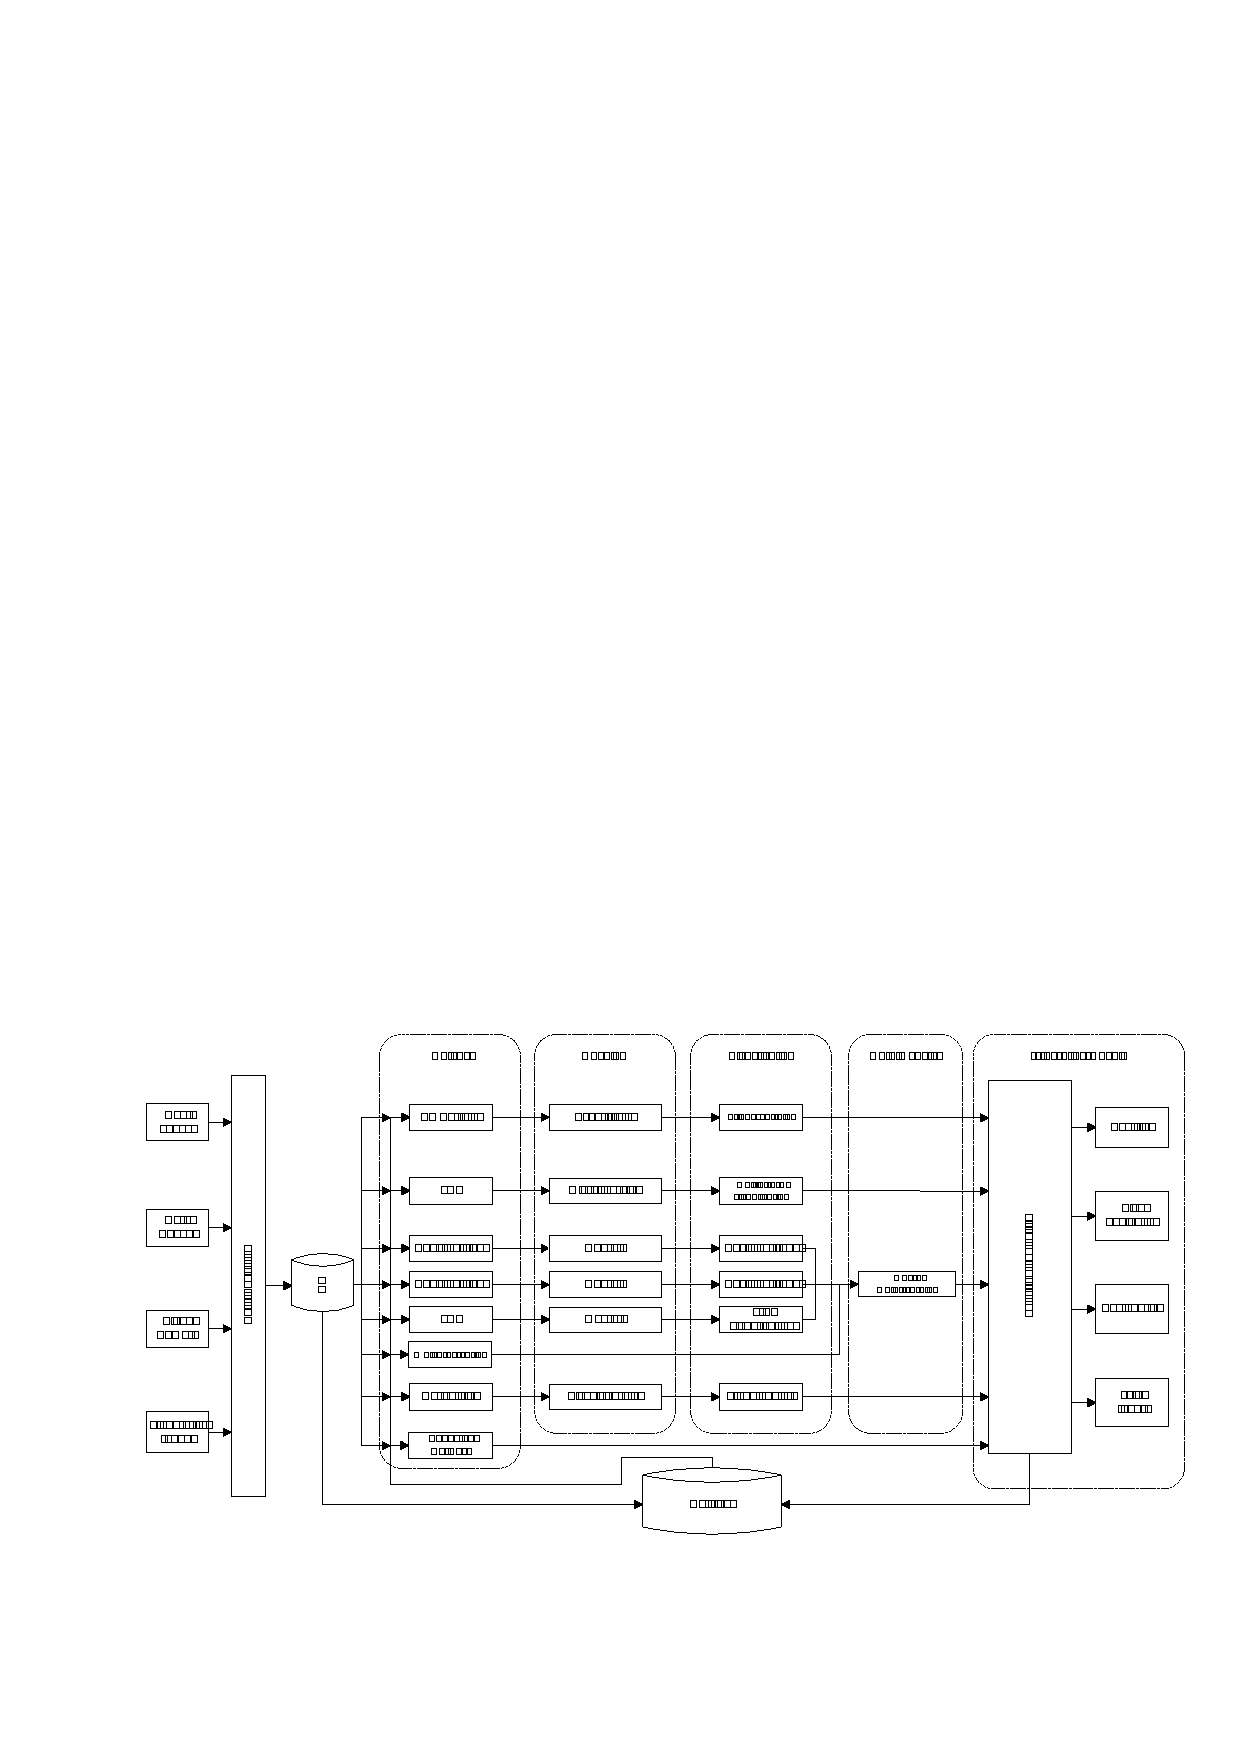
\includegraphics[width=0.95\textheight, angle=90]{chap_security/shema.pdf}
\caption{Information flow in the implemented platform.}
\label{fig:implementation}
\end{figure}
%\clearpage

Based on the final probability, the entry was classified into one of the classes: \textit{OK}, for regular entry, and \textit{alarm}, for irregular entry.
The system ontology stored each module's evaluations and explanations. The platform is presented in Figure~\ref{fig:implementation}. 
%It comprehends information flow from peripheral sensors through modules, up to the final integration and reports available to the human operator. 


\subsection{Ontology}
\label{sec:ontology}

The modules and methods use the same or similar data while processing, and therefore require a comprehensible presentation. Besides the basic relationships between pieces of information, such as the sensor's value, complex representations are also required; for example, a sensor \textit{belongs to} an access point.

We have developed an ontology using the Web Ontology Language (OWL) \citep{Horrocks03} and the ontology editor \cite{Protege}. 
The ontology consists of a central part, including event data and its classifications, and several local parts, each of them storing particular module knowledge. The central part includes information about: 
\begin{itemize}
    \item  	access points: position, security requirements etc; 
    \item 	persons: personal details, position in a company, rooms of the building that a person has permission to enter etc; 
    \item 	sensors: type; for example, biometric sensor, sensor access point;   
    \item 	events: person who produced the event, access point where it was produced, event sensors, individual module and final classification, and actions enabled via evaluation.
\end{itemize}

The ontology structure ensures knowledge of the system and its setting in a flexible presentation. This means that new sensors, modules, and access points can be easily added.





%%%%%%%%%%%%%%%%%%%%%%%%%%%%%%%%%%%%%%%%%%%%%%%%%%%%%%%%%%%%%%%%%%%%%%%
%
% M O D U L E S
%
%%%%%%%%%%%%%%%%%%%%%%%%%%%%%%%%%%%%%%%%%%%%%%%%%%%%%%%%%%%%%%%%%%%%%%%

\section{Detectors}
\label{sec:modules}

\index{detector}
This section describes the modules and algorithms in more detail. In this particular implementation, we prefer algorithms that can provide as much of an explanation as possible, but in general, it is possible to select any learning algorithm.


\subsection{Expert Rules Detector}
\label{sec:modules:rules}

The first module consists of expert rules defined by a security expert or a human operator. These rules do not learn from past person behavior; instead each rule has adjustable parameters, enabling new rule creation by specifying the rule-parameter values. 
The rules are described in the SWRL language \citep{W3Cswrl} for querying data stored in the OWL. A test over the events is performed by the Jess rule engine \citep{Jess}. 

We have implemented two types of rules. If the entry procedure is violated, the first rule type triggers an alarm independently of the other modules. The second rule type refers to the entry observation; for example, \textit{``The person accessed this area more than five times in the past two minutes''}. Instead of unconditionally triggering an alarm, each triggered rule $R_i$ returns a probability $\Prob\{R_i\}$ that the entry is regular. If several second-type rules $R_1, \dots, R_n$ are triggered, then $min(\Prob\{R_1\}, \dots, \Prob\{R_n\})$ is returned and the module composes an explanation consisting of the violated rules and their parameters. Otherwise, if none of the rules is violated, the entry is regular according to the rules, and, therefore, the returned probability $p$ equals $1$.

An example of the second-type SWRL rule is shown in Figure~\ref{fig:SWRL}.
\begin{figure}[]
\centering
\begin{verbatim}


event(?event_object) & swrl_end_of_testing(?event_object, ?event_swrl) &
swrlb:equal(?event_swrl, false) & card_time(?event_object, ?time_of_event) &
swrlb:greaterThan(?time_of_event,  "18:00:00") &
swrlb:lessThan(?time_of_event, "7:00:00")
THEN
swrl_rules_result(?event_object, "0.0") &
swrl_rules_explanation(?event_object, ?event_swrl_explanation) &
swrlb:stringConcat(?event_swrl_explanation, 
                   "Alarm: event time is between 18:00 and 7:00")
\end{verbatim}
\caption{An expert-rule example written in SWRL.}
\label{fig:SWRL}
\end{figure}
The rule queries events that occurred between 6:00pm and 7:00am and marks these events as alarms, since events are not allowed at night.



\subsection{Micro-Movement Detector}
\label{sec:modules:micro}

The micro-learning module learns short-term behavior. The attributes are calculated as three time differences from four input times:
\begin{eqnarray}
   \Delta t_1 &=& t_f-t_c, \\
    \Delta t_2 &=& t_{do}-t_f, \\
    \Delta t_3 &=& t_{dc}-t_{do}.
\end{eqnarray}
Each observation $\mathbf{x}_i$ is thus represented by a triple $\mathbf{x}_i=(\Delta t_{i,1},\Delta t_{i,2},\Delta t_{i,3})$. All the regular entries of a particular person form a learning set $\mathcal{X}=\{\mathbf{x}_1,\mathbf{x}_2,\dots ,\mathbf{x}_n\}$. When the person produces a new observation $\mathbf{x}_{n+k}$, the module compares it with the learning set $\mathcal{X}$ and returns an outlier factor: if the new observation is similar to the existing observations, $\mathbf{x}_{n+k}$ is a regular observation with a low outlier factor; otherwise, it is an outlier with a high outlier factor.

In previous work, \cite{Tusar2006} examined various outlier detection algorithms, selected the LOF (Local Outlier Factor, \citep{Breunig2001}) and implemented it. The algorithm reportedly achieves reliable performance where instances are not uniformly distributed in the attribute space. 
The LOF for a new observation $\mathbf{x}_i$ is defined as 
\begin{equation}
LOF_k (\mathbf{x}_i )=\frac{1}{|ngb_k (\mathbf{x}_i,\mathcal{X})|} * \sum_{\mathbf{y} \in ngb_k(\mathbf{x}_i,\mathcal{X})} \frac{ldns_k(\mathbf{y})}{ldns_k (\mathbf{x}_i)},
\end{equation}
where $ngb(\mathbf{x}_i,\mathcal{X})$ is the set of $k$-nearest neighbors of the observation $\mathbf{x}_i$, and $ldns_k(\mathbf{y})$ is the local density of an observation $\mathbf{y}$ and its $k$ nearest neighbors. Intuitively, $LOF_k (\mathbf{x}_i ) \leq 1$ when the new observation is near an existing cluster within $\mathcal{X}$, and $LOF_k (\mathbf{x}_i )  >1$ when the observation is far from the cluster.

The final outputs of the module are the LOF value, the probability that the entry is regular, and a visual explanation. The probability is computed from the LOF value using the following procedure. Let $\tau_l < 1$ denote the regular entry threshold value and let $\tau_u > 1$ denote the irregular entry threshold value. Then, the probability $\Prob\{\mathbf{x}\}$ that the entry $\mathbf{x}$ is regular is computed as a linear threshold values combination:
\begin{equation}
   p(e) =  \begin{cases} 
1.0 & \text{if } LOF(e) \leq \tau_l, \\
0.0 & \text{if } LOF(e) \geq \tau_u, \\
\frac{\tau_u-LOF(e)}{\tau_u-\tau_l} & \text{otherwise}.
\end{cases}
\end{equation}


%\frac{b_u-LOF}{b_u-b_l} \text{otherwise} \\

Since the module uses only three micro-attributes, its visualization can be presented in a three-dimensional space, with one dimension for each attribute. The entries are thus presented as points, and the each point's LOF value is represented by a color: red for outliers, yellow for unclear entries, and green for regular clustered entries. Figure~\ref{fig:microLOF} shows an entry cluster in a learning set $\mathcal{X}$ (circles) and a new entry $\mathbf{x}_i$ (a plus).


\begin{figure}[]
\centering
%\includegraphics[type=eps,ext=.eps,read=.eps,width=8cm]{chap_security/mikro1}
%\includegraphics[bb=45 75 375 270, width=8cm]{chap_security/mikro1}
\includegraphics[width=0.9\linewidth]{chap_security/mikro1}
\caption{Regular entries of a particular person (circles) and a new entry denoted as an outlier ('+').}
\label{fig:microLOF}
\end{figure}


\subsection{Macro-Movement and Meta-Detector}
\label{sec:modules:macro}

The macro-level data are used in three modules, two of which also exploit the micro-level data. The macro-level attributes are divided into two groups describing a current entry and the relation between the current entry and previous entries. The attributes from the first group are, for example, the current time and date, the day of the week, the date in relation to the month (that is, the second Friday in the month). The second group defines such relations as the number of previous entries in the same day (for the current person), the person who entered previously in a specific time interval, the entry time on the same day in the previous week, etc. 
It is important to note that macro-learning would be more powerful if we had monitored more than one access point.

The first macro-module learns only from macro-attributes. The positive learning examples are a person's regular entries, while the negative learning examples are a person's  irregular entries and the entries of other persons. Several machine-learning algorithms were tested and, finally, decision trees were selected,  Weka's J48 implementation of C4.5, in particular \citep{Witten2005}. The main decision tree benefit is the ability to explain a decision after classification. The path leading from the root to the chosen leaf is colored according to the classification: green for regular entries and red for alarms. Target variable distribution in the chosen leaf is interpreted as the probability that the entry is regular. The classification problem was introduced as a verification, where each person has his/her own decision tree with two possible outcomes: true, if the claimed identity is valid, and false otherwise.

The second macro-module applies the same algorithm as the previous module, but uses both micro- and macro-attributes. While the first macro-module considers only macro-level behavior and discovers patterns, for example, \textit{``User X comes to work on Mondays between 8.15 and 8.40~(93\%)''}, the second macro-module refines these patterns by incorporating micro-attributes.

\index{local outlier factor, LOF}
In the third macro-module, the macro- and micro-attributes are used for learning with the LOF algorithm. In contrast to the micro-module, where the visualization was intuitive, the large number of attributes requires a different representation. For this purpose, we implemented parallel coordinate visualization. Each attribute is presented on one vertical axis, ranging from the minimum to the maximum normalized value. Thus, each entry is represented as a broken line intersecting the attribute value coordinates. The line is colored according to the entry's LOF value: green for regular entries, yellow for unclear entries, and red otherwise. Figure~\ref{fig:macroLOF} shows a cluster of learning set entries and the new entry as a dotted line.

\begin{figure}[]
\centering
%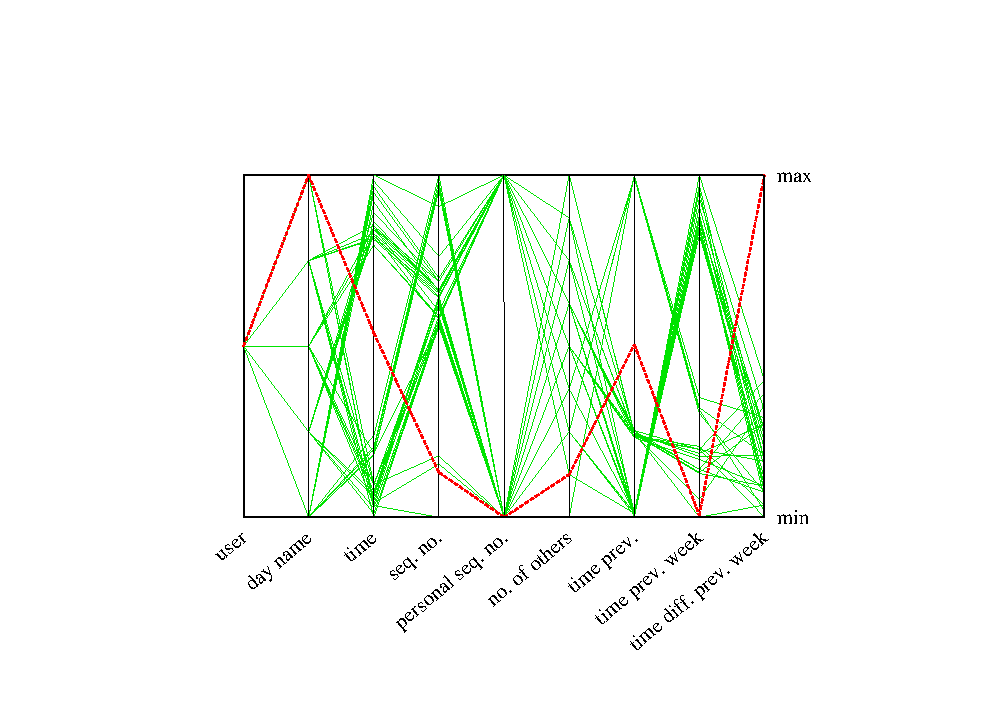
\includegraphics[type=eps,ext=.eps,read=.eps,width=8cm]{chap_security/makro-lof}
%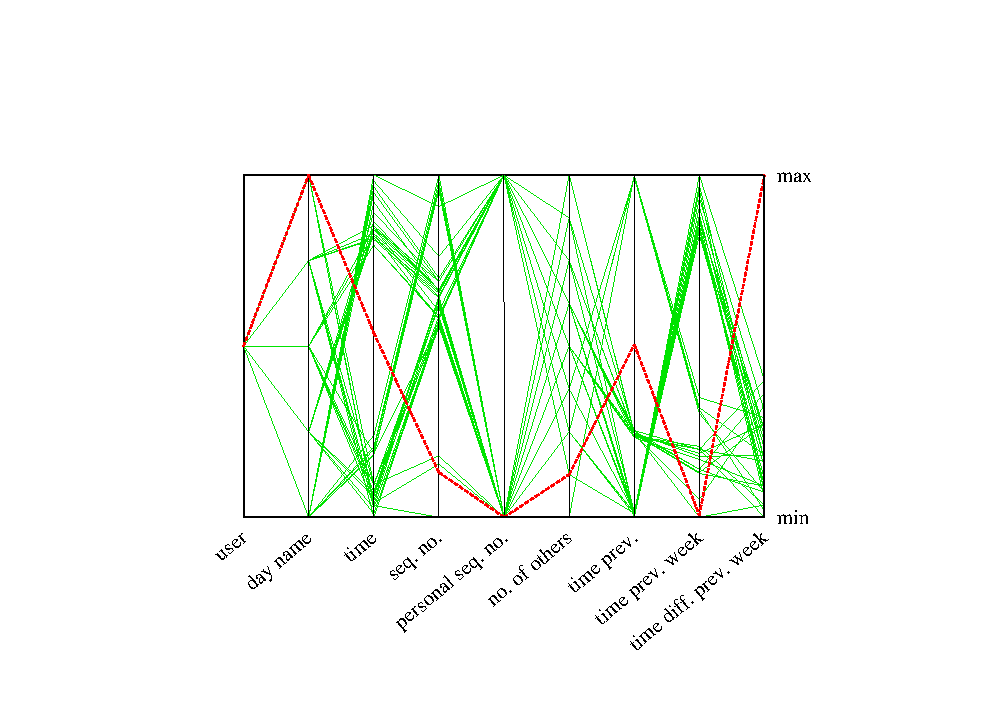
\includegraphics[bb=80 50 390 300,width=8cm]{chap_security/makro-lof}
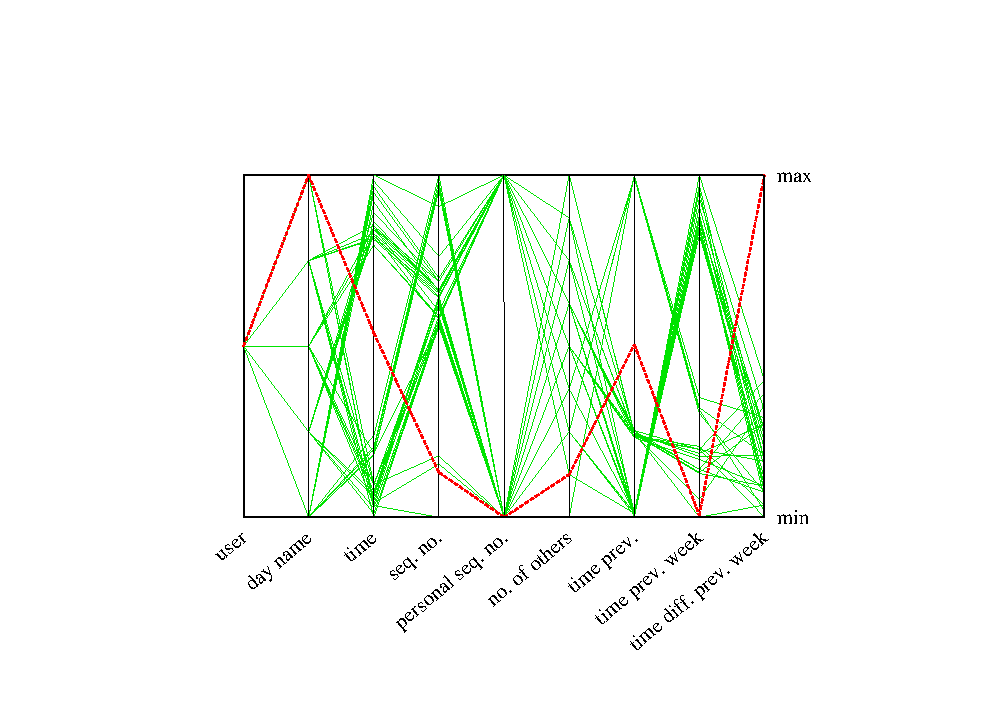
\includegraphics[width=0.7\linewidth]{chap_security/makro-lof}
\caption{Multi-dimensional representation of regular entries (thin lines) and a new entry (dotted line) classified as an alarm. There are nine attributes with values normalized between the minimum and maximum values.}
\label{fig:macroLOF}
\end{figure}


Finally, the macro-meta-module combines the classifications of all three macro-modules. Then, all the results and visualizations are written into the ontology. %In the tested prototype, only weighted voting was implemented; however, several meta-level learning algorithms were applied later. 
Also, in the tested implementation, only the macro-meta-learning was applied, but in principle, an arbitrary subgroup of modules could be connected using meta-learners. 

\subsection{Visual Detector}
\label{sec:modules:visual}

The visual learning module developed by \cite{pers2007} learns person movement patterns using an access point video camera and classifies a new entry as either regular or not. For this purpose, a web camera with a $1.3$ Mpixel resolution and 30-fps rate was used.

When a new entry occurs, the last 30 seconds of video are analyzed in the following steps: first, the optical flow histograms are computed and divided into six segments, approximating body parts. Next, in each segment, the prevailing movement is estimated and transferred into a sequence of symbols. This sequence defines the movement's digital signature and is used for the verification. Each person has a learning set of valid regular entries, which are compared with the new entry signatures. Finally, the module outputs the classification and probability that the entry is regular as a normalized comparison. 

It should be noted that other sensor analyses, such as speech or walking patterns, could be added as well.

\subsection{Multimodal Detector Integration}
\label{sec:modules:integration} 
	
After the expert rules, micro-learning, macro-learning, meta-learning, and visual-learning have made their assessments, their results are integrated into a current entry joint risk analysis. It estimates the event probability $\Prob\{$\textit{entry $|$ entry is regular}$\}$ given the module observations. If the estimated probability does not exceed a threshold value, an alarm is triggered. Note that an alarm can also be triggered by expert rules when there is sufficient certainty.

The reasoning in the prototype system is performed with a Bayesian network, structured as shown in Figure~\ref{fig:bayesianNetwork}. Four modules have a direct impact on the entry event; that is, expert rules, micro-learning and visual learning, and a macro-meta-learning module, while the macro-meta-learning module depends only on the three macro-modules. The network probabilities are computed from the train dataset, using the \textit{m-estimate} for conditional probabilities and the \textit{Laplace estimate} for a-priori probabilities. 
\begin{figure}[]
\centering
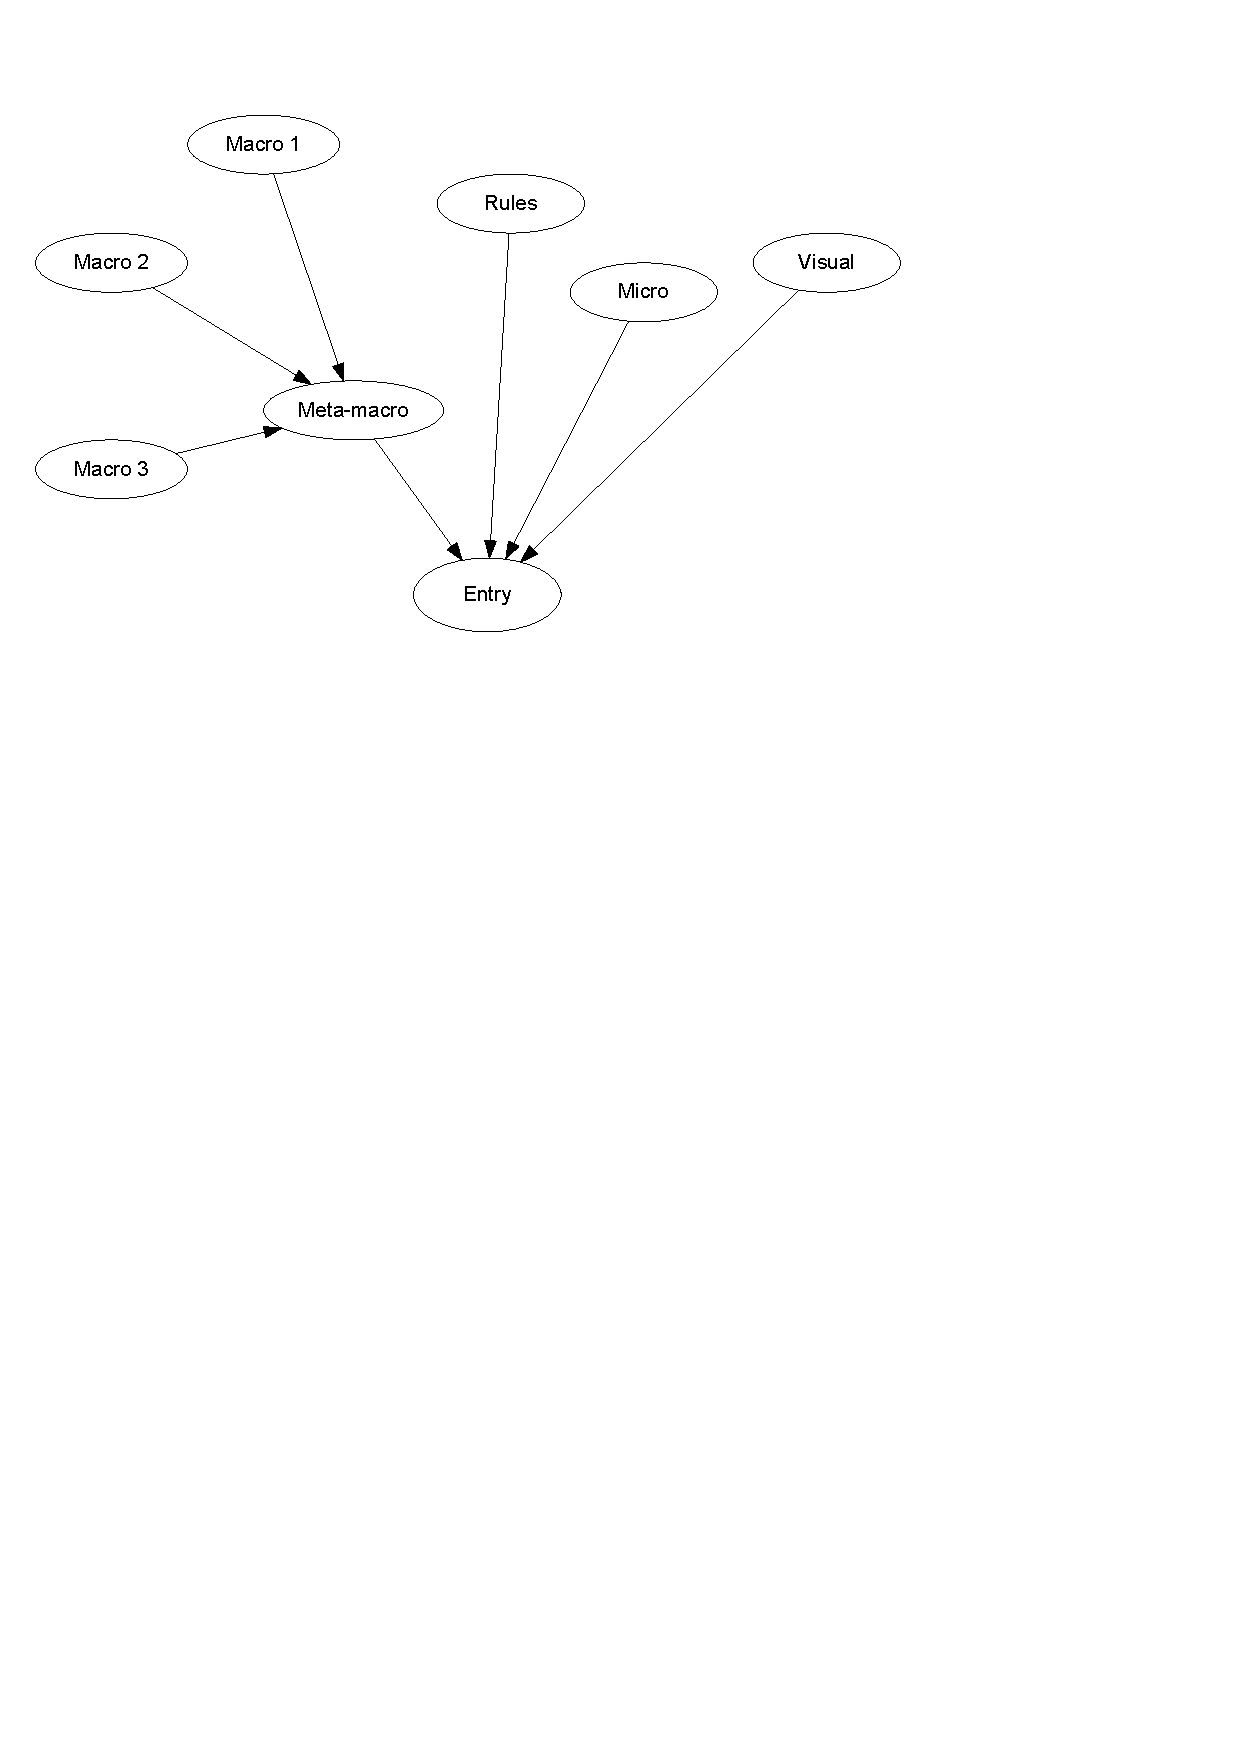
\includegraphics[width=0.8\linewidth]{chap_security/BayesNetwork2}
%\includegraphics[bb=30 590 360 820,width=8cm]{chap_security/BayesNetwork.pdf}
%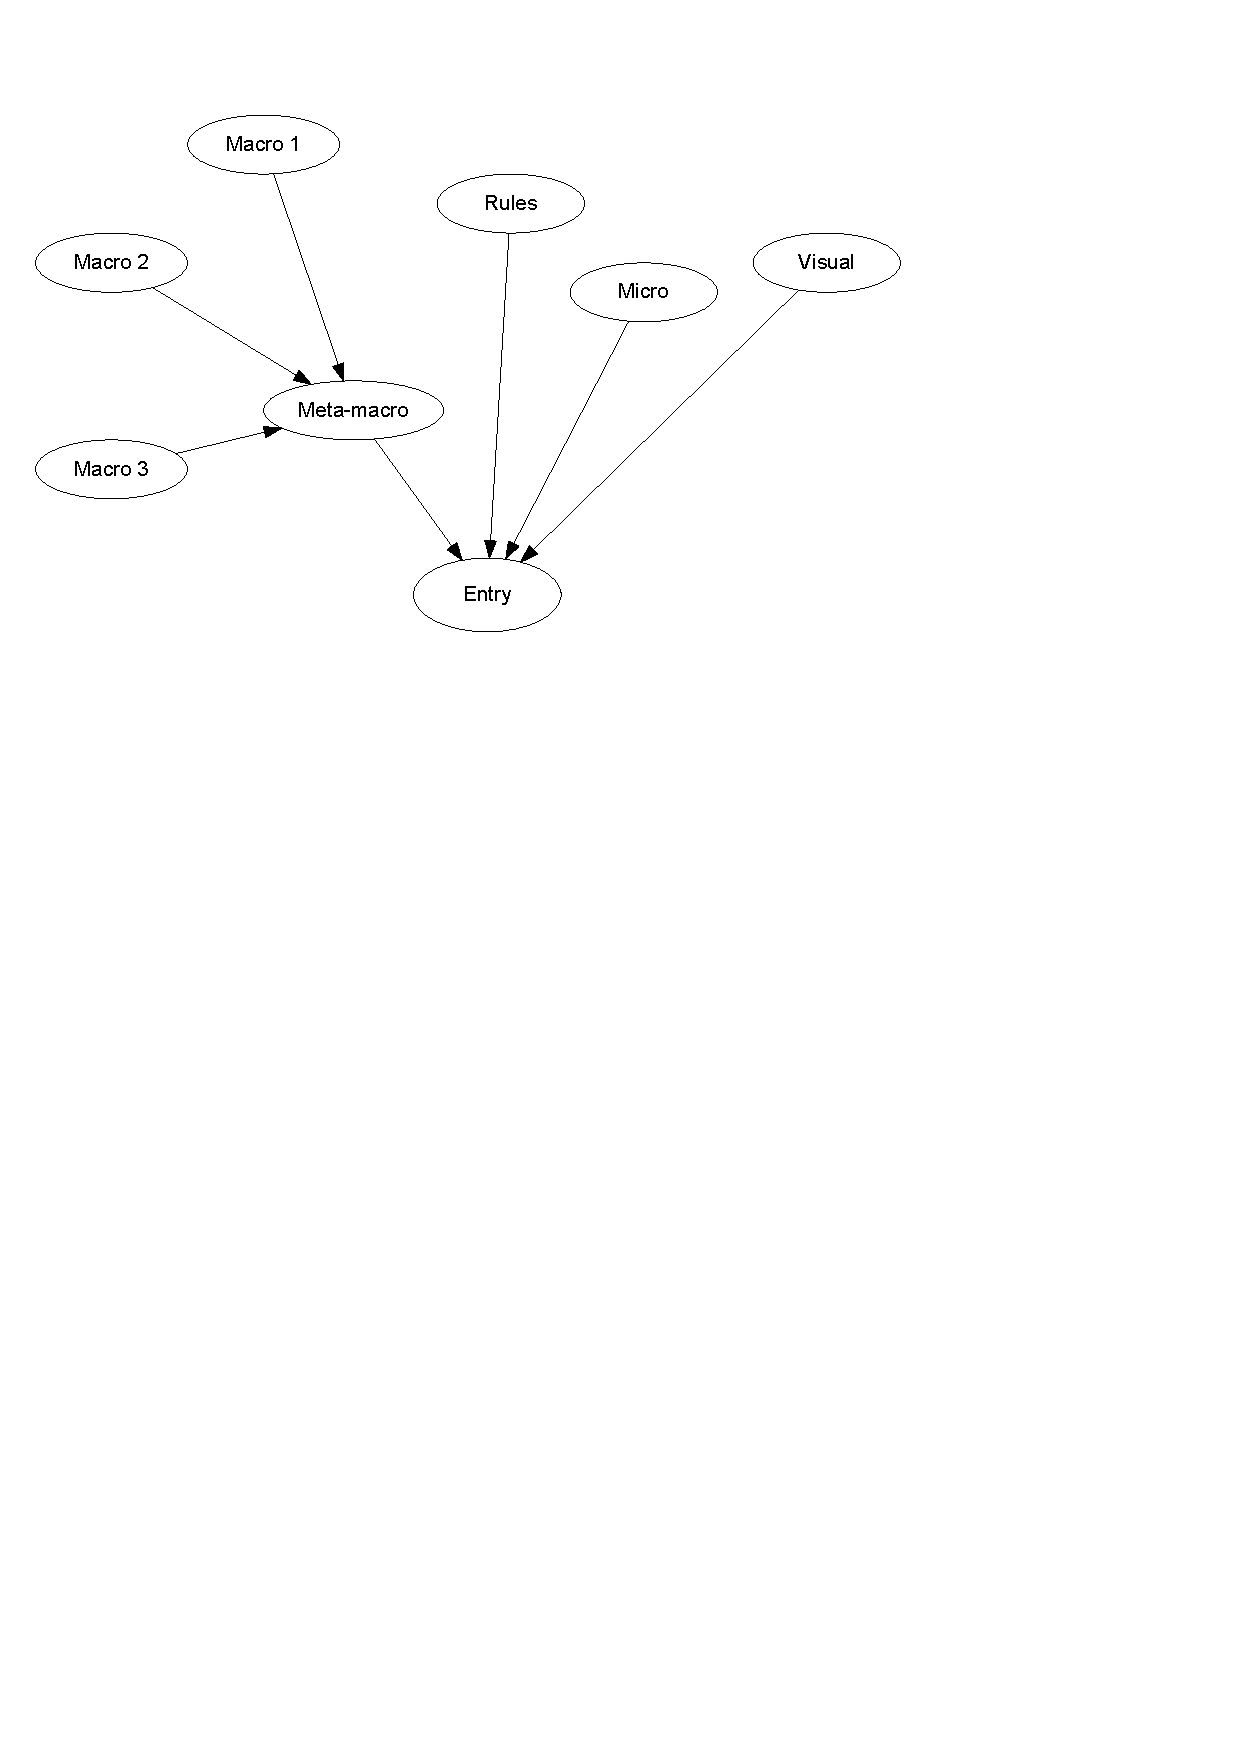
\includegraphics[bb=0 540 440 800,width=8cm]{chap_security/BayesNetwork2.pdf}
\caption{Bayesian network used for reasoning.}
\label{fig:bayesianNetwork}
\end{figure}

The integration proceeds in three steps. Firstly, the output from each module is converted to interval the $[0, 1]$ representing the a-posteriori probability $\Prob\{M_i\}$ that the entry event is regular. Secondly, given the Bayesian network and the probabilities $\Prob\{M_i\}$, the estimated  probability of an entry event is computed from the network.
%\begin{eqnarray}
%P(E | M_1, M_2, \dots, M_n) = P(E) \frac{P(M_1, M_2, \dots, M_n | E)}{P(M_1, M_2, \dots, M_n)}
%\end{eqnarray}
%Numerator is developed with chain rule and due to the structure of the network is simplified to:
%\begin{multline}
%P(M_1, M_2, \dots, M_n | E) = \prod_{i=1}^{n} P(M_i | Parents(M_i)) = \\
% = \prod_{i=1}^{n} p_{M_i} P(M_i=1|E) + (1-p_{M_i}) P(M_i=0|E)
%\end{multline}
%Denominator, on the other hand, is independent of the event E, thus is developed as follows:
%\begin{multline}
%P(M_1, M_2, \dots, M_n) = \\
% = \sum_{e\in\{0, 1\}} P(E=e) P(M_1, M_2, \dots, M_n | E=e)  =\\
% = \sum_{e\in\{0, 1\}} P(E=e) \prod_{i=1}^{n} (p_{M_i} P(M_i=1|E=e) + \\
% + (1-p_{M_i}) P(M_i=0|E=e))
%\end{multline}

Finally, the integration module outputs the joint analysis as a probability that the entry is regular and provides an explanation. According to the threshold values, the integration module triggers \textit{alarm} or \textit{OK} and stores the results in the ontology. In high-security areas, the cost of a false alarm is negligible compared to the cost of an unrecognized intruder; therefore, the system is set to minimize the latter.



%%%%%%%%%%%%%%%%%%%%%%%%%%%%%%%%%%%%%%%%%%%%%%%%%%%%%%%%%%%%%%%%%%%%%%%
%
% E X P E R I M E N T A L   R E S U L T S
%
%%%%%%%%%%%%%%%%%%%%%%%%%%%%%%%%%%%%%%%%%%%%%%%%%%%%%%%%%%%%%%%%%%%%%%%

\section{Experimental Results}
\label{sec:results}
  



An experimental verification was performed in the prototype environment as described in Section~\ref{sec:system:experimental}. It consisted of learning and evaluation phases. In this chapter, we report on one learning and three evaluation experiments.

\subsection{Learning Phase}
In the learning phase, four people were recorded accessing the system. Each individual completed 40 regular entries that were used as positive learning examples. The negative learning examples for one individual were the entries of the other three people. We built decision trees for the macro-modules, constructed learning sets for the LOF algorithm in the micro-and macro-module and a comparison set for the visual learning module, and adjusted the system parameters. After the learning was completed, the system was ready to operate. 


\subsection{Evaluation Phase}
In the evaluation phase, we performed three experiments: two with simulated entries and one real-time experiment with security experts. 

The first two experiments were performed off-line with simulated tests. The focus was on a \textit{fake-identity} scenario, where an adversary has stolen an employee's identity. We recorded the regular entries of four people in the role of an employee (the system already knew them) and three people in the role of an intruder (new to the system). Each person made 31 regular entries, serving as the testing examples. Both experiments were tested without the visual learning since it did not allow offline testing. Consequently, the Bayesian network for the integration was slightly changed, omitting the visual learning module. The experiments were run on already-learned and tuned modules from the learning phase, while the Bayesian network probabilities were obtained with a 10-fold cross-validation.

In the first experiment, the identities of the employees were swapped. We took four employees that were known to the system and shuffled their identities in order to simulate a scenario where an employee hands over his/her identity. The dataset contained 496 examples with a distribution of 75\% negative examples (fake identity). 

The system and the module performance in the first experiment is presented in Table~\ref{tab:dataset1}. The first two columns represent irregular entries, where employee identity was swapped, and regular entries with the correct employee identity. Each number denotes an accuracy; for example, the left-most number represents the irregular entry percentage predicted as regular by the expert rules. The last column presents the overall module accuracy. The system achieved an overall accuracy of 95.77\%. The expert rules always predicted \textit{OK}, because all the entries were formally regular according to the entry procedure. The micro-learning detected both irregular and regular entries well, while the macro-learning had 10.08\% more mistakes. The high accuracy of the micro-module was expected because it is relatively easy to distinguish the movement of a couple of people given sufficient learning examples.

In the second experiment, we used the intruders' entries, which were unknown to the system, and assigned them the employees' identities. In this way, we simulated a stolen-identity scenario. The dataset consisted of 496 examples with a distribution 75\% of negative examples.

The second experiment measurements are shown in Table~\ref{tab:dataset2}. The system achieved an overall accuracy of 96.57\%. In contrast with the results in Table~\ref{tab:dataset1}, where macro-learning classified 16.13\% false positives, the number of false positives in Table~\ref{tab:dataset2} is only 1.88\%. However, the trend in the micro-learning is just the opposite; the overall accuracy is comparable in both datasets. The decline in micro-learning performance was to be expected, since it is more difficult to classify new, unseen behavior than to distinguish between known cases.

\begin{table}[!ht]
\centering

\begin{tabular}{cccccc}
\toprule
\multicolumn{ 1}{c}{} &                   \multicolumn{ 4}{c}{Scenarios} &            \\
%\hline
		& \multicolumn{ 2}{c}{Irregular entries} & \multicolumn{ 2}{c}{Regular entries} &   Overall  \\
 		&   {\it OK} & {\it alarm} &   {\it OK} & {\it alarm} &   Accuracy \\
Modules	&   [\%] & [\%] &   [\%] & [\%] &  [\%] \\
\hline
Expert rules &   100.00 &     0.00 &   100.00 &     0.00 &    25.00 \\

Micro learning &     5.91 &    94.09 &    92.74 &     7.26 &    93.75 \\

Macro learning &    16.13 &    83.87 &    83.06 &    16.94 &    83.67 \\
\hline
Integration &     1.08 &    98.92 &    86.29 &    13.71 &    95.77 \\
\toprule
\end{tabular}  
 
\caption{System and module performance in the offline \textit{swapped identity} experiment with four employees only.}
\label{tab:dataset1}
\end{table}

\begin{table}[!ht]
\centering

\begin{tabular}{cccccc}
\toprule
\multicolumn{ 1}{c}{} &                   \multicolumn{ 4}{c}{Scenarios} &            \\
%\hline
		& \multicolumn{ 2}{c}{Irregular entries} & \multicolumn{ 2}{c}{Regular entries} &   Overall  \\
 		&   {\it OK} & {\it alarm} &   {\it OK} & {\it alarm} &   Accuracy \\
Modules	&   [\%] & [\%] &   [\%] & [\%] &  [\%] \\
\hline
Expert rules &   100.00 &     0.00 &   100.00 &     0.00 &    25.00 \\

Micro learning &    22.04 &    77.96 &    92.74 &     7.26 &    81.65 \\

Macro learning &     1.88 &    98.12 &    82.26 &    17.74 &    94.15 \\
\hline
Integration &     0.00 &   100.00 &    86.29 &    13.71 &    96.57 \\
\toprule
\end{tabular}  
  
 
\caption{System and module performance in the offline \textit{stolen identity} experiment with four employees and three intruders.}
\label{tab:dataset2}
\end{table}

In the third, most relevant experiment, we invited security experts from the Slovenian Ministry of Defense to test the system with a live simulation of various security attacks.  For the purpose of scientific experimentation, the following eight scenarios were proposed, tested and executed live by the experts:
\begin{enumerate}
    \item regular entry: a person enters normally;
    \item unusual time: the access time is out of normal working hours or on a non-working day;
    \item multiple entries: a person regularly accesses a secure room several times in a short period of time;
    \item unusual behavior: a person is under threat or in a strange state of mind;
    \item tailgating: two persons access a secure room using a single identity;
    \item burglary: an attacker disables the hardware protection by force;
    \item fake identity: an attacker accesses a secure room with a stolen identity card and a forged fingerprint;
    \item kidnapping: an attacker forces an employee to enable secure room access.
\end{enumerate}
Each scenario was imitated several times by different persons and in a different order, as requested by the security experts. In total, 45 irregular entries and 15 regular entries were performed. The video learning module was active.

The results described in Table~\ref{tab:results} are separated into two groups: regular entries (scenario 1) and irregular entries (scenarios 2-8). The numbers show the percentage of test examples classified as \textit{OK}, \textit{alarm} or \textit{failed} by the corresponding module. The classification may fail due to the disabling of sensors (for example, the burglary scenario).


\begin{table}[!ht]
\centering

\begin{tabular}{ccccccc}
\toprule
           &                                \multicolumn{ 5}{c}{Scenarios} &            \\
%\hline
		   & \multicolumn{ 3}{c}{Irregular entries} & \multicolumn{ 2}{c}{Regular entries} &   Overall  \\
           &   {\it OK} & {\it alarm} & {\it failed} &   {\it OK} & {\it alarm} &   Accuracy \\
Modules    &   [\%] 	& [\%] & [\%] &   [\%] & [\%] &  [\%] \\
\hline
Expert rules &    84.44 &    15.56 &     0.00 &   100.00 &     0.00 &    36.67 \\

Micro learning &     0.00 &    88.89 &    11.11 &    93.33 &     6.67 &    90.00 \\

Macro learning &     0.00 &    88.89 &    11.11 &    86.67 &    13.33 &    88.33 \\

Visual learning &     8.89 &    88.89 &     4.44 &    73.33 &    26.67 &    85.00 \\

Integration &     0.00 &   100.00 &     0.00 &    86.67 &    13.33 &    96.67 \\
\toprule
\end{tabular}  


\caption{System and module performance in the experiments with four employees and four  security experts in a role of intruder.}
\label{tab:results}
\end{table}

The system achieved an overall accuracy of 96.67\%, identifying all the irregular entries, and being too suspicious of two regular entries. Once again, the expert rules classified with a low accuracy (36.67\%), but when an entry was classified as an alarm, it was indeed so. The rules were more robust compared to the other modules, which, for example, failed to recognize the burglary scenario. The micro- and macro-learning modules recognized the irregular entries with the same accuracy, but macro-learning made more mistakes when classifying the regular entries. It should be noted that all the tests were performed within two hours, which is not well suited to macro-learning. The visual learning was slightly more robust (that is, less failures) than the learning modules, but achieved a lower accuracy. 





%%%%%%%%%%%%%%%%%%%%%%%%%%%%%%%%%%%%%%%%%%%%%%%%%%%%%%%%%%%%%%%%%%%%%%%
%
% C O N C L U S I O N
%
%%%%%%%%%%%%%%%%%%%%%%%%%%%%%%%%%%%%%%%%%%%%%%%%%%%%%%%%%%%%%%%%%%%%%%%
\section{Discussion}
\label{sec:conclusion}

We have designed a modular, intelligent system for analyzing access point intrusion risk. The system, in principle, combines an arbitrary number of intelligent modules on  top of an arbitrary number of physical devices. The emphasis is on modeling the behavior of the regular person and estimating the risk that a new entry is not regular, based on meta-learning and integration. 

In a practical evaluation\footnote{A short video of the third experiment is available online:\\http://www.youtube.com/watch?v=BNDgfFRQkU4.} we presented three experiments, which demonstrated encouraging results.
It was clear that each module has its own strong and weak points. However, an advanced combination and integration overcomes the individual weaknesses and combines different aspects into a reliable risk evaluation. For example, if we had used only the best module (micro-learning) in the third experiment, the achieved accuracy would have been 90.00\%, while the default accuracy (which is rather meaningless) would have been 75.00\%. The accuracy of the integrated system was 96.67\%.

In each system, there is a fine line between being too sensitive and not being sensitive enough to small changes in behavior. Although some of the methods, for example, the Bayesian network, are quite robust, any practical application needs some fine tuning of the system parameters. One of the first major benchmarks painfully reminded us of the difference between a laboratory test and a field test; that is, one of the early system versions was able to successfully distinguish between normal persons, but security experts found a way to trick the intelligent modules. Only after incorporating  some modifications, was the system able to cope with human expertise, as presented in Table~\ref{tab:results}.

One of the system drawbacks is that it requires a learning procedure: the system can be used only after a certain amount of regular accesses have been made. Furthermore, if a person changes behavior, for example, due to an injury, the learning must start anew. Further work on the system must include a mechanism for continuous learning and person adaptation over time.

The complex methods implemented seem to be excessive for a simple commercial application. In its current form, the system is more appropriate for high-security areas. Namely, the joint-verification methods turned out to be very hard to bypass. A single method can be fooled relatively easily, but deceiving different methods within a normal time interval is a much harder task. 

In summary, intelligent access-point risk analysis represents an improvement and has the potential to demonstrate this in real-time applications.


%\section*{Acknowledgment}
%This study has received funding, partly from the Slovenian Ministry of Defense (MORS) and partly from the Slovenian Research Agency (ARRS). The authors also thank the 20 members of the project team, in particular Jana Krivec, Robert Blatnik and Ale{\v s} Tav{\v c}ar, as well as the security experts and supervisors.